\thispagestyle{appendixheader}
\stepcounter{app}
\setcounter{app_fig}{1}
\setcounter{app_tab}{1}
\setcounter{equation}{0}
\renewcommand\theequation{附\arabic{app}-\arabic{equation}}
% \renewcommand\theequation{\Alph{app}.\arabic{equation}}
\renewcommand\chaptername{附录}
\renewcommand\chaptername{Appendix} 
\renewcommand\thechapter{附录\zhnum{app}} 

\setcounter{chapter}{0}
\setcounter{section}{0}
\chapter{附录中的公式}\label{chap:app1}{

对公式的引用如,公式\eqref{eq:appedns}
\begin{equation} \label{eq:appedns}
    % \adddotsbeforeeqnnum%
    \begin{cases}
        \frac{\partial \rho}{\partial t} + \nabla\cdot(\rho\Vector{V}) = 0\\
        \frac{\partial (\rho\Vector{V})}{\partial t} + \nabla\cdot(\rho\Vector{V}\Vector{V}) = \nabla\cdot\Tensor{\sigma}\\
        \frac{\partial (\rho E)}{\partial t} + \nabla\cdot(\rho E\Vector{V}) = \nabla\cdot(k\nabla T) + \nabla\cdot(\Tensor{\sigma}\cdot\Vector{V})
    \end{cases}
\end{equation}

\begin{equation} \label{eq:appedns2}
    % \adddotsbeforeeqnnum%
    \begin{cases}
        \frac{\partial \rho}{\partial t} + \nabla\cdot(\rho\Vector{V}) = 0\\
        \frac{\partial (\rho\Vector{V})}{\partial t} + \nabla\cdot(\rho\Vector{V}\Vector{V}) = \nabla\cdot\Tensor{\sigma}\\
        \frac{\partial (\rho E)}{\partial t} + \nabla\cdot(\rho E\Vector{V}) = \nabla\cdot(k\nabla T) + \nabla\cdot(\Tensor{\sigma}\cdot\Vector{V})
    \end{cases}
\end{equation}


mathtext: $A,F,L,2,3,5,\sigma$, mathnormal: $A,F,L,2,3,5,\sigma$, mathrm: $\mathrm{A,F,L,2,3,5,\sigma}$.

mathbf: $\mathbf{A,F,L,2,3,5,\sigma}$, mathit: $\mathit{A,F,L,2,3,5,\sigma}$, mathsf: $\mathsf{A,F,L,2,3,5,\sigma}$.

mathtt: $\mathtt{A,F,L,2,3,5,\sigma}$, mathfrak: $\mathfrak{A,F,L,2,3,5,\sigma}$, mathbb: $\mathbb{A,F,L,2,3,5,\sigma}$.

mathcal: $\mathcal{A,F,L,2,3,5,\sigma}$, mathscr: $\mathscr{A,F,L,2,3,5,\sigma}$, boldsymbol: $\boldsymbol{A,F,L,2,3,5,\sigma}$.

vector: $\Vector{\sigma, T, a, F, n}$, unitvector: $\unitVector{\sigma, T, a, F, n}$

matrix: $\Matrix{\sigma, T, a, F, n}$, unitmatrix: $\unitMatrix{\sigma, T, a, F, n}$

tensor: $\Tensor{\sigma, T, a, F, n}$, unittensor: $\unitTensor{\sigma, T, a, F, n}$ 


\thispagestyle{appendixheader}
}
\chapter{附录中的图表}{
\stepcounter{app}
\setcounter{app_fig}{1}
\setcounter{app_tab}{1}


附表测试

\begin{apptab}[!htbp]
    \bicaption{\enspace 这是一个样表}{\enspace This is a sample table}
    \stepcounter{app_tab}
    \label{apptab:1}
    \centering
    \footnotesize% fontsize
    \setlength{\tabcolsep}{4pt}% column separation
    \renewcommand{\arraystretch}{1.2}%row space 
    \begin{tabular}{lcccccccc}
        \hline
        行号 & \multicolumn{8}{c}{跨多列的标题}\\
        %\cline{2-9}% partial hline from column i to column j
        \hline
        Row 1 & $1$ & $2$ & $3$ & $4$ & $5$ & $6$ & $7$ & $8$\\
        \hline
    \end{tabular}
\end{apptab}


\begin{apptab}[!htbp]
    \bicaption{\enspace 这是一个样表}{\enspace This is a sample table}
    \stepcounter{app_tab}
    \label{apptab:2}
    \centering
    \footnotesize% fontsize
    \setlength{\tabcolsep}{4pt}% column separation
    \renewcommand{\arraystretch}{1.2}%row space 
    \begin{tabular}{lcccccccc}
        \hline
        行号 & \multicolumn{8}{c}{跨多列的标题}\\
        %\cline{2-9}% partial hline from column i to column j
        \hline
        Row 1 & $1$ & $2$ & $3$ & $4$ & $5$ & $6$ & $7$ & $8$\\
        \hline
    \end{tabular}
\end{apptab}

附图测试

\begin{appfig}[!htbp]
    \centering
    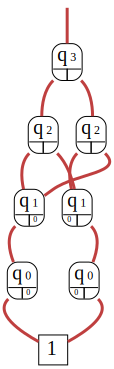
\includegraphics[width=0.40\textwidth]{Img/cx}
    \bicaption{\enspace 这是一个样图}{\enspace This is a sample figure}
    \fignote{对图片的注释}
    
    \label{appfig:1}
    \stepcounter{app_fig}
\end{appfig}

% //TODO: 是否需要附录
}